\section{Methods}
	This section gives an overview of the methods used to conduct this study. It is structured chronologically in the sense of data processing steps (see also figure X). First, the potential data sources are introduced. Second, the process of harvesting the images used to train ICARUS is explained, as well as the methods used to train the algorithm. In the third subsection validation procedures used are shown. The fourth part explains how ICARUS was run. The final section covers how the results form running ICARUS were mapped.
	\bigskip
	
	Explain Flowchart here
	
	\bigskip
	
	\begin{figure}
        \centering
	    


\tikzset{every picture/.style={line width=0.75pt}} %set default line width to 0.75pt        

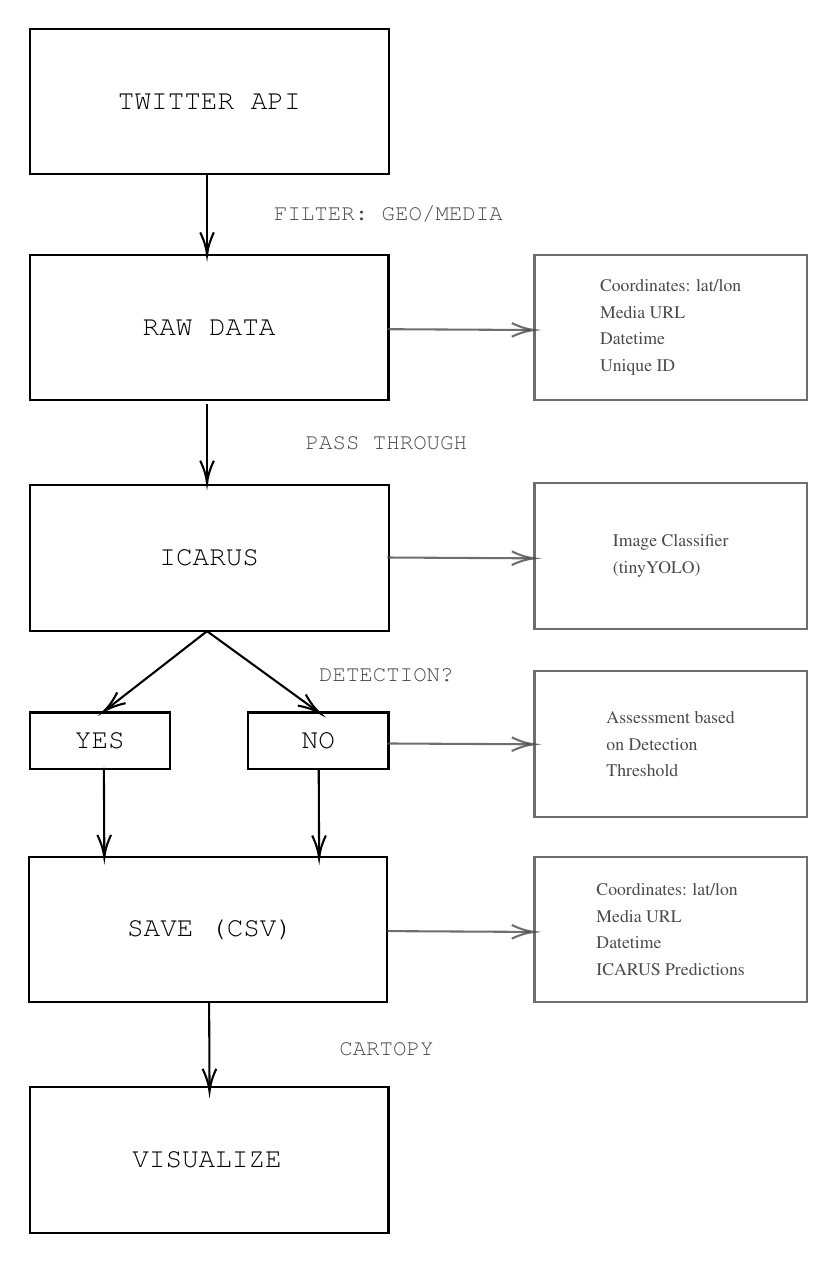
\begin{tikzpicture}[x=0.75pt,y=0.75pt,yscale=-1,xscale=1]
%uncomment if require: \path (0,660); %set diagram left start at 0, and has height of 660

%Flowchart: Process [id:dp3971687376584736] 
\draw   (199.68,60.33) -- (372.52,60.33) -- (372.52,130.33) -- (199.68,130.33) -- cycle ;
%Straight Lines [id:da3722057941016612] 
\draw    (285.02,130.6) -- (285.02,167.4) ;
\draw [shift={(285.02,169.4)}, rotate = 270] [color={rgb, 255:red, 0; green, 0; blue, 0 }  ][line width=0.75]    (10.93,-3.29) .. controls (6.95,-1.4) and (3.31,-0.3) .. (0,0) .. controls (3.31,0.3) and (6.95,1.4) .. (10.93,3.29)   ;

%Flowchart: Process [id:dp7915450261326966] 
\draw   (199.6,169.33) -- (372.43,169.33) -- (372.43,239.33) -- (199.6,239.33) -- cycle ;
%Flowchart: Process [id:dp31890687546180385] 
\draw   (199.68,280.33) -- (372.52,280.33) -- (372.52,350.33) -- (199.68,350.33) -- cycle ;
%Flowchart: Process [id:dp1798468479163131] 
\draw   (199.1,459.33) -- (371.93,459.33) -- (371.93,529.33) -- (199.1,529.33) -- cycle ;
%Flowchart: Process [id:dp8194881297537675] 
\draw   (199.6,389.79) -- (267.18,389.79) -- (267.18,417.17) -- (199.6,417.17) -- cycle ;
%Flowchart: Process [id:dp5454108064950349] 
\draw   (199.6,570.33) -- (372.43,570.33) -- (372.43,640.33) -- (199.6,640.33) -- cycle ;
%Flowchart: Process [id:dp3149621536877212] 
\draw   (304.85,389.79) -- (372.43,389.79) -- (372.43,417.17) -- (304.85,417.17) -- cycle ;
%Straight Lines [id:da3000291100753305] 
\draw    (285.02,241) -- (285.02,277.4) ;
\draw [shift={(285.02,279.4)}, rotate = 270] [color={rgb, 255:red, 0; green, 0; blue, 0 }  ][line width=0.75]    (10.93,-3.29) .. controls (6.95,-1.4) and (3.31,-0.3) .. (0,0) .. controls (3.31,0.3) and (6.95,1.4) .. (10.93,3.29)   ;

%Straight Lines [id:da3779446467217289] 
\draw    (235.32,416.5) -- (235.51,457.7) ;
\draw [shift={(235.52,459.7)}, rotate = 269.73] [color={rgb, 255:red, 0; green, 0; blue, 0 }  ][line width=0.75]    (10.93,-3.29) .. controls (6.95,-1.4) and (3.31,-0.3) .. (0,0) .. controls (3.31,0.3) and (6.95,1.4) .. (10.93,3.29)   ;

%Straight Lines [id:da5478043110101576] 
\draw    (338.82,416.8) -- (339.01,458) ;
\draw [shift={(339.02,460)}, rotate = 269.73] [color={rgb, 255:red, 0; green, 0; blue, 0 }  ][line width=0.75]    (10.93,-3.29) .. controls (6.95,-1.4) and (3.31,-0.3) .. (0,0) .. controls (3.31,0.3) and (6.95,1.4) .. (10.93,3.29)   ;

%Straight Lines [id:da36668666505152103] 
\draw    (286.02,529.2) -- (286.21,570.4) ;
\draw [shift={(286.22,572.4)}, rotate = 269.73] [color={rgb, 255:red, 0; green, 0; blue, 0 }  ][line width=0.75]    (10.93,-3.29) .. controls (6.95,-1.4) and (3.31,-0.3) .. (0,0) .. controls (3.31,0.3) and (6.95,1.4) .. (10.93,3.29)   ;

%Straight Lines [id:da9485100671630313] 
\draw    (285.02,350.6) -- (236.7,388.17) ;
\draw [shift={(235.12,389.4)}, rotate = 322.13] [color={rgb, 255:red, 0; green, 0; blue, 0 }  ][line width=0.75]    (10.93,-3.29) .. controls (6.95,-1.4) and (3.31,-0.3) .. (0,0) .. controls (3.31,0.3) and (6.95,1.4) .. (10.93,3.29)   ;

%Straight Lines [id:da9817319309154029] 
\draw    (285.02,350.6) -- (337.9,389.02) ;
\draw [shift={(339.52,390.2)}, rotate = 216] [color={rgb, 255:red, 0; green, 0; blue, 0 }  ][line width=0.75]    (10.93,-3.29) .. controls (6.95,-1.4) and (3.31,-0.3) .. (0,0) .. controls (3.31,0.3) and (6.95,1.4) .. (10.93,3.29)   ;

%Flowchart: Process [id:dp8914422903741139] 
\draw  [color={rgb, 255:red, 74; green, 74; blue, 74 }  ,draw opacity=0.8 ] (442.77,169.33) -- (574.02,169.33) -- (574.02,239.33) -- (442.77,239.33) -- cycle ;
%Flowchart: Process [id:dp3094514982649226] 
\draw  [color={rgb, 255:red, 74; green, 74; blue, 74 }  ,draw opacity=0.8 ] (442.77,279.4) -- (574.02,279.4) -- (574.02,349.4) -- (442.77,349.4) -- cycle ;
%Flowchart: Process [id:dp6350575730299324] 
\draw  [color={rgb, 255:red, 74; green, 74; blue, 74 }  ,draw opacity=0.8 ] (442.77,459.33) -- (574.02,459.33) -- (574.02,529.33) -- (442.77,529.33) -- cycle ;
%Flowchart: Process [id:dp4180968434721368] 
\draw  [color={rgb, 255:red, 74; green, 74; blue, 74 }  ,draw opacity=0.8 ] (442.77,370) -- (574.02,370) -- (574.02,440) -- (442.77,440) -- cycle ;
%Straight Lines [id:da5306027300225034] 
\draw [color={rgb, 255:red, 74; green, 74; blue, 74 }  ,draw opacity=0.8 ]   (371.93,315.1) -- (440.77,315.49) ;
\draw [shift={(442.77,315.5)}, rotate = 180.32] [color={rgb, 255:red, 74; green, 74; blue, 74 }  ,draw opacity=0.8 ][line width=0.75]    (10.93,-3.29) .. controls (6.95,-1.4) and (3.31,-0.3) .. (0,0) .. controls (3.31,0.3) and (6.95,1.4) .. (10.93,3.29)   ;

%Straight Lines [id:da6129943654827146] 
\draw [color={rgb, 255:red, 74; green, 74; blue, 74 }  ,draw opacity=0.8 ]   (371.93,205.1) -- (440.77,205.49) ;
\draw [shift={(442.77,205.5)}, rotate = 180.32] [color={rgb, 255:red, 74; green, 74; blue, 74 }  ,draw opacity=0.8 ][line width=0.75]    (10.93,-3.29) .. controls (6.95,-1.4) and (3.31,-0.3) .. (0,0) .. controls (3.31,0.3) and (6.95,1.4) .. (10.93,3.29)   ;

%Straight Lines [id:da06735980977616274] 
\draw [color={rgb, 255:red, 74; green, 74; blue, 74 }  ,draw opacity=0.8 ]   (371.93,404.7) -- (440.77,405.09) ;
\draw [shift={(442.77,405.1)}, rotate = 180.32] [color={rgb, 255:red, 74; green, 74; blue, 74 }  ,draw opacity=0.8 ][line width=0.75]    (10.93,-3.29) .. controls (6.95,-1.4) and (3.31,-0.3) .. (0,0) .. controls (3.31,0.3) and (6.95,1.4) .. (10.93,3.29)   ;

%Straight Lines [id:da1328641994921984] 
\draw [color={rgb, 255:red, 74; green, 74; blue, 74 }  ,draw opacity=0.8 ]   (371.93,495.1) -- (440.77,495.49) ;
\draw [shift={(442.77,495.5)}, rotate = 180.32] [color={rgb, 255:red, 74; green, 74; blue, 74 }  ,draw opacity=0.8 ][line width=0.75]    (10.93,-3.29) .. controls (6.95,-1.4) and (3.31,-0.3) .. (0,0) .. controls (3.31,0.3) and (6.95,1.4) .. (10.93,3.29)   ;


% Text Node
\draw (286.1,95.33) node  [align=left] {{\fontfamily{pcr}\selectfont TWITTER API}};
% Text Node
\draw (372.43,149.8) node [scale=0.9,color={rgb, 255:red, 74; green, 74; blue, 74 }  ,opacity=1 ] [align=left] {{\fontfamily{pcr}\selectfont {\small FILTER: GEO/MEDIA}}};
% Text Node
\draw (371.43,260) node [scale=0.9,color={rgb, 255:red, 74; green, 74; blue, 74 }  ,opacity=1 ] [align=left] {{\fontfamily{pcr}\selectfont {\small PASS THROUGH}}};
% Text Node
\draw (371.43,372) node [scale=0.9,color={rgb, 255:red, 74; green, 74; blue, 74 }  ,opacity=1 ] [align=left] {{\fontfamily{pcr}\selectfont {\small DETECTION?}}};
% Text Node
\draw (371.43,551.8) node [scale=0.9,color={rgb, 255:red, 74; green, 74; blue, 74 }  ,opacity=1 ] [align=left] {{\fontfamily{pcr}\selectfont {\small CARTOPY}}};
% Text Node
\draw (286.02,204.33) node  [align=left] {{\fontfamily{pcr}\selectfont RAW DATA}};
% Text Node
\draw (286.1,315.33) node  [align=left] {{\fontfamily{pcr}\selectfont ICARUS}};
% Text Node
\draw (286.52,494.33) node  [align=left] {{\fontfamily{pcr}\selectfont SAVE (CSV)}};
% Text Node
\draw (233.39,403.48) node  [align=left] {{\fontfamily{pcr}\selectfont YES}};
% Text Node
\draw (338.64,403.48) node  [align=left] {{\fontfamily{pcr}\selectfont NO}};
% Text Node
\draw (285.02,605.33) node  [align=left] {{\fontfamily{pcr}\selectfont VISUALIZE}};
% Text Node
\draw (508.39,204.33) node [scale=0.8,color={rgb, 255:red, 74; green, 74; blue, 74 }  ,opacity=1 ] [align=left] {{\footnotesize {\fontfamily{ptm}\selectfont Coordinates: lat/lon}}\\{\footnotesize {\fontfamily{ptm}\selectfont Media URL}}\\{\footnotesize {\fontfamily{ptm}\selectfont Datetime}}\\{\footnotesize {\fontfamily{ptm}\selectfont Unique ID}}};
% Text Node
\draw (508.39,314.4) node [scale=0.8,color={rgb, 255:red, 74; green, 74; blue, 74 }  ,opacity=1 ] [align=left] {{\footnotesize {\fontfamily{ptm}\selectfont Image Classifier}}\\{\footnotesize {\fontfamily{ptm}\selectfont (tinyYOLO)}}};
% Text Node
\draw (508.39,405) node [scale=0.8,color={rgb, 255:red, 74; green, 74; blue, 74 }  ,opacity=1 ] [align=left] {{\fontfamily{ptm}\selectfont {\footnotesize Assessment based}}\\{\fontfamily{ptm}\selectfont {\footnotesize on Detection }}\\{\fontfamily{ptm}\selectfont {\footnotesize Threshold}}};
% Text Node
\draw (508.39,494.33) node [scale=0.8,color={rgb, 255:red, 74; green, 74; blue, 74 }  ,opacity=1 ] [align=left] {{\fontfamily{ptm}\selectfont {\footnotesize Coordinates: lat/lon}}\\{\fontfamily{ptm}\selectfont {\footnotesize Media URL}}\\{\fontfamily{ptm}\selectfont {\footnotesize Datetime}}\\{\fontfamily{ptm}\selectfont {\footnotesize ICARUS Predictions}}};


\end{tikzpicture}

	    \caption{Flowchart of Methodology.}
	\end{figure}

	\bigskip
	
	\newpage
	    
	    \subsection{Data Source(s)}
		\subsection{Harvesting of Training Images}
		\subsection{Supervised Classification & Training of ICARUS}
		\subsection{Validation}
		    \subsubsection{Mean Average Precision}
		    \subsubsection{Validation with Google Streetview}
		\subsection{Running ICARUS}
		    \subsubsection{Gathering Actual Data}
		    \subsubsection{Processing with ICARUS}
		\subsubsection{Visualization}
